%%%%%%%%%%%%%%%%%%%%%%%%%%%%%%%%%%%%%%%%%
% Structured General Purpose Assignment
% LaTeX Template
%
% This template has been downloaded from:
% http://www.latextemplates.com
%
% Original author:
% Ted Pavlic (http://www.tedpavlic.com)
%
% Note:
% The \lipsum[#] commands throughout this template generate dummy text
% to fill the template out. These commands should all be removed when 
% writing assignment content.
%
%%%%%%%%%%%%%%%%%%%%%%%%%%%%%%%%%%%%%%%%%

%----------------------------------------------------------------------------------------
%	PACKAGES AND OTHER DOCUMENT CONFIGURATIONS
%----------------------------------------------------------------------------------------

\documentclass{article}

\usepackage{fancyhdr} % Required for custom headers
\usepackage{lastpage} % Required to determine the last page for the footer
\usepackage{extramarks} % Required for headers and footers
\usepackage{graphicx} % Required to insert images
\usepackage{lipsum} % Used for inserting dummy 'Lorem ipsum' text into the template
\usepackage{enumerate}
\usepackage{booktabs}
\usepackage{amsmath}
\usepackage{booktabs}

% Margins
\topmargin=-0.45in
\evensidemargin=0in
\oddsidemargin=0in
\textwidth=6.5in
\textheight=9.0in
\headsep=0.25in 

\linespread{1.5} % Line spacing

% Set up the header and footer
\pagestyle{fancy}
\lhead{\hmwkAuthorName} % Top left header
\chead{\hmwkClass\ (\hmwkTitle)} % Top center header
%%\rhead{\firstxmark} 
\rhead{} % Top right header
\lfoot{\lastxmark} % Bottom left footer
\cfoot{} % Bottom center footer
\rfoot{Page\ \thepage\ of\ \pageref{LastPage}} % Bottom right footer
\renewcommand\headrulewidth{0.4pt} % Size of the header rule
\renewcommand\footrulewidth{0.4pt} % Size of the footer rule

\setlength\parindent{0pt} % Removes all indentation from paragraphs

%----------------------------------------------------------------------------------------
%	DOCUMENT STRUCTURE COMMANDS
%	Skip this unless you know what you're doing
%----------------------------------------------------------------------------------------

% Header and footer for when a page split occurs within a problem environment
\newcommand{\enterProblemHeader}[1]{
\nobreak\extramarks{#1}{#1 continued on next page\ldots}\nobreak
\nobreak\extramarks{#1 (continued)}{#1 continued on next page\ldots}\nobreak
}

% Header and footer for when a page split occurs between problem environments
\newcommand{\exitProblemHeader}[1]{
\nobreak\extramarks{#1 (continued)}{#1 continued on next page\ldots}\nobreak
\nobreak\extramarks{#1}{}\nobreak
}

\setcounter{secnumdepth}{0} % Removes default section numbers
\newcounter{homeworkProblemCounter} % Creates a counter to keep track of the number of problems

\newcommand{\homeworkProblemName}{}
\newenvironment{homeworkProblem}[1][Question \arabic{homeworkProblemCounter}]{ % Makes a new environment called homeworkProblem which takes 1 argument (custom name) but the default is "Question #"
\stepcounter{homeworkProblemCounter} % Increase counter for number of problems
\renewcommand{\homeworkProblemName}{#1} % Assign \homeworkProblemName the name of the problem
\section{\homeworkProblemName} % Make a section in the document with the custom problem count
\enterProblemHeader{\homeworkProblemName} % Header and footer within the environment
}{
\exitProblemHeader{\homeworkProblemName} % Header and footer after the environment
}

\newcommand{\problemAnswer}[1]{ % Defines the problem answer command with the content as the only argument
\noindent\framebox[\columnwidth][c]{\begin{minipage}{0.98\columnwidth}#1\end{minipage}} % Makes the box around the problem answer and puts the content inside
}

\newcommand{\homeworkSectionName}{}
\newenvironment{homeworkSection}[1]{ % New environment for sections within homework problems, takes 1 argument - the name of the section
\renewcommand{\homeworkSectionName}{#1} % Assign \homeworkSectionName to the name of the section from the environment argument
\subsection{\homeworkSectionName} % Make a subsection with the custom name of the subsection
\enterProblemHeader{\homeworkProblemName\ [\homeworkSectionName]} % Header and footer within the environment
}{
\enterProblemHeader{\homeworkProblemName} % Header and footer after the environment
}

%----------------------------------------------------------------------------------------
%	EXPECTATION AND VARIANCE OPERATOR
%----------------------------------------------------------------------------------------
 \newcommand{\E}{\mathrm{E}} 
 \newcommand{\Var}{\mathrm{Var}}
 \newcommand{\Cov}{\mathrm{Cov}}
 \newcommand{\Corr}{\mathrm{Corr}}
 
%----------------------------------------------------------------------------------------
%	NAME AND CLASS SECTION
%----------------------------------------------------------------------------------------

\newcommand{\hmwkTitle}{Problem Set\ \#1} % Assignment title
\newcommand{\hmwkDueDate}{Wednesday,\ February\ 7,\ 2018} % Due date
\newcommand{\hmwkClass}{FIN\ 521} % Course/class
\newcommand{\hmwkClassTime}{2:00pm} % Class/lecture time
\newcommand{\hmwkAuthorName}{Wanbae Park} % Your name

%----------------------------------------------------------------------------------------
%	TITLE PAGE
%----------------------------------------------------------------------------------------

\title{
\vspace{2in}
\textmd{\textbf{\hmwkClass:\ \hmwkTitle}}\\
\normalsize\vspace{0.1in}\small{Due\ on\ \hmwkDueDate}\\
\vspace{3in}
}

\author{\textbf{\hmwkAuthorName}}
\date{} % Insert date here if you want it to appear below your name

%----------------------------------------------------------------------------------------

\begin{document}

\maketitle

%----------------------------------------------------------------------------------------
%	TABLE OF CONTENTS
%----------------------------------------------------------------------------------------

%\setcounter{tocdepth}{1} % Uncomment this line if you don't want subsections listed in the ToC

%%\newpage
%%\tableofcontents
\newpage

%----------------------------------------------------------------------------------------
%	QUESTION 1
%----------------------------------------------------------------------------------------
\begin{homeworkProblem}
	Ratios stated on the problem set are calculated as follows.
	\begin{enumerate}[a.]
		\item Market/Book = Market Capitalization / Book value of equity
		\item Interest coverage = Some measure of income(operating income, EBIT, EBITDA ...) / Interest payments
		\item EV/EBITDA = Enterprise value / EBITDA = Market value of equity + Debt - Cash / EBITDA
		\item Market leverage = Debt / Equity
		\item Current ratio = Current assets / Current liabilities
	\end{enumerate}
	Table \ref{tab:q1-ratios} shows numerical values of ratios calculated by using data from Global Corp's financial statement.
%----------------------------------------------------------------------------------------	
	%% Table of ratios
	\begin{table}[h]
	\centering
	\begin{tabular}{@{}cccccc@{}}
	\toprule
                           & \multicolumn{2}{c}{Definition}          & \multicolumn{3}{c}{Numerical Values} \\ \midrule
	Name of Ratio              & Numerator        & Denominator          & Numerator   & Denominator   & Ratio  \\ \midrule
	\textit{Market/Book}       & Market Cap.      & Book value of equity & 36          & 22.2          & 1.62   \\
	\textit{Interest Coverage} & Operating income & Interest payments    & 10.4        & 7.7           & 1.35   \\
	\textit{EV/EBITDA}         & Enterprise value & EBITDA               & 131.5       & 11.6          & 11.34  \\
	\textit{Market Leverage}   & Debt             & Equity               & 147.9       & 170.1         & 0.87   \\
	\textit{Current Ratio}     & Current assets   & Current liabilities  & 57          & 34.7          & 1.64   \\ \bottomrule
	\end{tabular}
	\caption{Financial ratios of Global Corp. (Unit: million dollars)}
	\label{tab:q1-ratios}
	\end{table}
%----------------------------------------------------------------------------------------	
\end{homeworkProblem}
%----------------------------------------------------------------------------------------	
%----------------------------------------------------------------------------------------
%	QUESTION 2
%----------------------------------------------------------------------------------------
\begin{homeworkProblem}
	\begin{enumerate}[a.]
		\item In this case, \$20 million of cash would be credited, and same amount of long-term debt would be debited. Since the same amount of account in balance sheet have been offset, there is no change in Global's book value of equity.
		\item Inventory would decrease by \$5 million, and there would be also a decrease of book value of equity by \$5 million.
		\item Since the firm used cash and long-term debt to purchase building, cash amount of \$5 million would be credited, long-term debt amount of \$5 million would be credited, and \$10 million amount of PP\&E would be debited. Since the amount of credited and debited balance sheet account is exactly equal, there is no change in Global's book value of equity.
		\item Because there is no possibility that Global would ever receive payment, there would be a decrease of accounts receivable by \$3 million dollars, as would the book value of equity.
		\item Reduction of cost might affect income statement. It might reduce cost of good sold. However, balance sheet of the firm does not change due to this event.
		\item The balance sheet does not change since the announcement of key competitor is not an economic event.
	\end{enumerate}
\end{homeworkProblem}
%----------------------------------------------------------------------------------------	
%----------------------------------------------------------------------------------------
%	QUESTION 3
%----------------------------------------------------------------------------------------
\begin{homeworkProblem}

\end{homeworkProblem}
%----------------------------------------------------------------------------------------	
%----------------------------------------------------------------------------------------
%	QUESTION 4
%----------------------------------------------------------------------------------------
\begin{homeworkProblem}
	According to the question, expected cash flow stream of the project is as follows.
%----------------------------------------------------------------------------------------	
	%% Cash Flow Table
	\begin{table}[h]
	\centering
	\begin{tabular}{@{}ccccccc@{}}
	\toprule
	\textit{Year}       & \textit{year 0} & \textit{year 1} & \textit{year 2} & \textit{year 3} & \textit{year 4} & \textit{year 5} \\
	\textit{Cash flows} & -10             & 5               & 2               & 2               & 2               & 2               \\ \bottomrule
	\end{tabular}
	\caption{Expected Cash Flows} \label{tab:q4-expected cf}
	\end{table}
%----------------------------------------------------------------------------------------	
	The payback period of this project is 4 years because cumulative cash flow from year 1 to year 4 is 11, and that from year 1 to year 3 is 10. That means it takes four years to retake the initial investment. If the required payback period is two years, the project is not accepted since the payback period is larger than required period. Since the cost of capital is given as 10\%, NPV of project is calculated as follows.
	\begin{equation*}	\label{eq:prob4-npv}
	\begin{aligned}
		NPV 		&= -10 + \frac{5}{(1+0.1)} + \frac{2}{(1+0.1)^2} + \frac{2}{(1+0.1)^3} + \frac{2}{(1+0.1)^4} + \frac{2}{(1 + 0.1)^5}	\\
				&= 0.309
	\end{aligned}
	\end{equation*}
	Therefore, the project has a positive NPV, and it means that the project is accepted if we use NPV rule.
\end{homeworkProblem}
%----------------------------------------------------------------------------------------	
%----------------------------------------------------------------------------------------
%	QUESTION 5
%----------------------------------------------------------------------------------------
\begin{homeworkProblem}
	\begin{figure}[h]
	\centering
		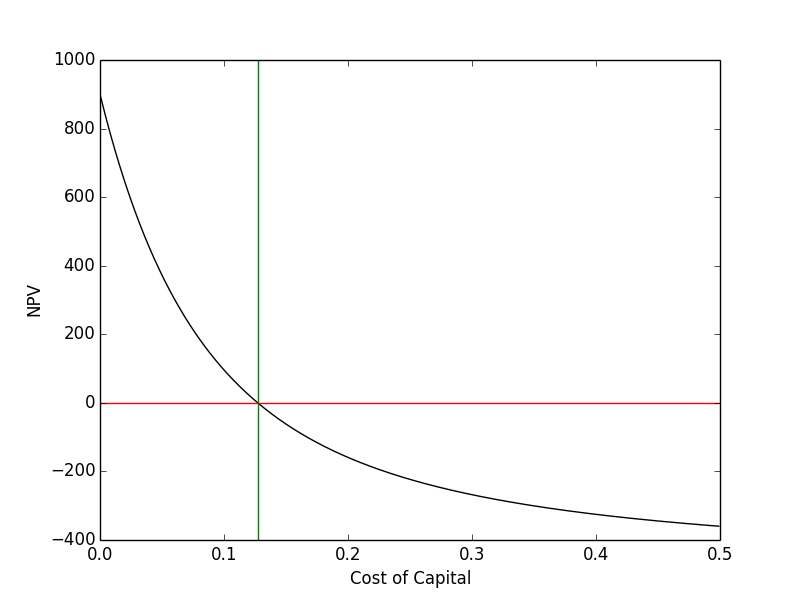
\includegraphics[scale = 0.7]{npv_plot.png}
		\caption{Plot of NPV}
	\end{figure}
\end{homeworkProblem}
\end{document}